\documentclass[tikz,border=3pt]{standalone}
\usepackage{amsmath}
\usepackage{tikz}
\usetikzlibrary{shapes.geometric,arrows.meta,patterns,calc}

\begin{document}
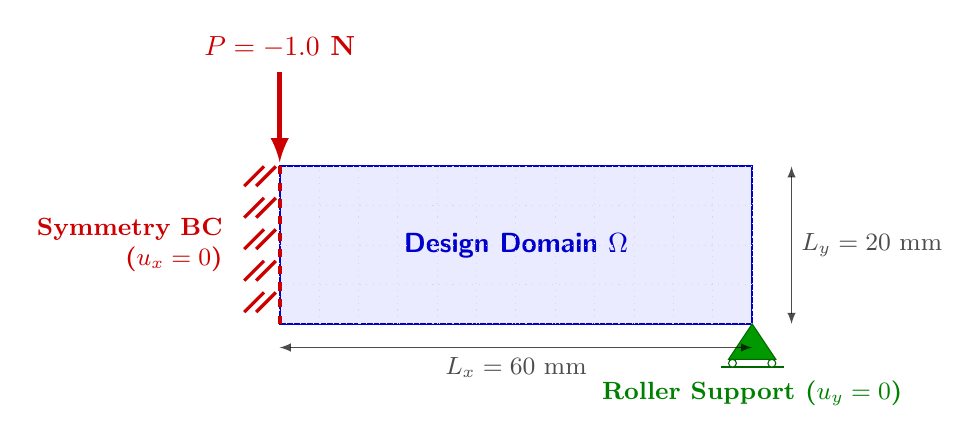
\begin{tikzpicture}[scale=1.0, >=latex]
  % Design Domain
  \draw[thick, fill=blue!8, draw=blue!80!black] (0,0) rectangle (6,2);
  \node[font=\bfseries\sffamily, color=blue!80!black] at (3,1) {Design Domain $\Omega$};
  
  % Grid overlay
  \draw[step=0.5, gray!30, dotted] (0,0) grid (6,2);
  
  % Symmetry Boundary Condition on Left Boundary (x=0)
  \draw[ultra thick, red!80!black, dashed] (0,0) -- (0,2);
  \foreach \y in {0.3, 0.7, 1.1, 1.5, 1.9} {
    \draw[line width=1.2pt, red!80!black] (-0.3, \y-0.15) -- (-0.05, \y+0.1);
    \draw[line width=1.2pt, red!80!black] (-0.45, \y-0.15) -- (-0.2, \y+0.1);
  }
  \node[left, red!80!black, font=\small\bfseries, align=right] at (-0.6, 1) {Symmetry BC\\($u_x = 0$)};
  
  % Roller Support at Bottom Right (6, 0)
  \draw[fill=green!60!black, draw=green!40!black] (6,0) -- (5.7, -0.45) -- (6.3, -0.45) -- cycle;
  \draw[thick, green!40!black] (5.6, -0.55) -- (6.4, -0.55);
  \draw[fill=white, draw=green!40!black] (5.75, -0.5) circle (0.05);
  \draw[fill=white, draw=green!40!black] (6.25, -0.5) circle (0.05);
  \node[below, green!50!black, font=\small\bfseries] at (6, -0.6) {Roller Support ($u_y = 0$)};
  
  % Concentrated Point Load at Top Left (0, 2)
  \draw[->, ultra thick, red!80!black, line width=2pt] (0, 3.2) -- (0, 2.05);
  \node[above, red!80!black, font=\bfseries] at (0, 3.25) {$P = -1.0\text{ N}$};
  
  % Dimensions
  \draw[<->, opacity=0.7] (0,-0.3) -- (6,-0.3) node[midway, below, font=\small] {$L_x = 60\text{ mm}$};
  \draw[<->, opacity=0.7] (6.5,0) -- (6.5,2) node[midway, right, font=\small] {$L_y = 20\text{ mm}$};
\end{tikzpicture}
\end{document}
